\section{Mathematical Formulation}
\label{sec:formulation}

\subsection{Physical Problem Description}
\label{subsec:problem}

A schematic of the physical configuration is shown in Figure~\ref{fig:schematic}. The domain is a two-dimensional, differentially heated, eccentric horizontal annulus. Unless stated otherwise, every length, temperature, and angular velocity given as a bare number in this paper is already non-dimensional, normalized as defined in Equation~\eqref{eq:nondim_vars} below. The outer cylinder is stationary, cooled, of non-dimensional radius $R_o = 0.5$, centered at the origin, held at non-dimensional temperature $\theta_o = 0$. The inner cylinder is heated, held at $\theta_i = 1$, of non-dimensional radius $R_i$ (varied across geometries), rotating about its own center at a fixed non-dimensional angular speed $\omega_i$, offset from the outer cylinder's center by a non-dimensional eccentricity $e$ along the vertical axis. The working fluid is air, $Pr = 0.71$, treated as incompressible and laminar under the Boussinesq approximation.

\begin{figure}[h]
\centering
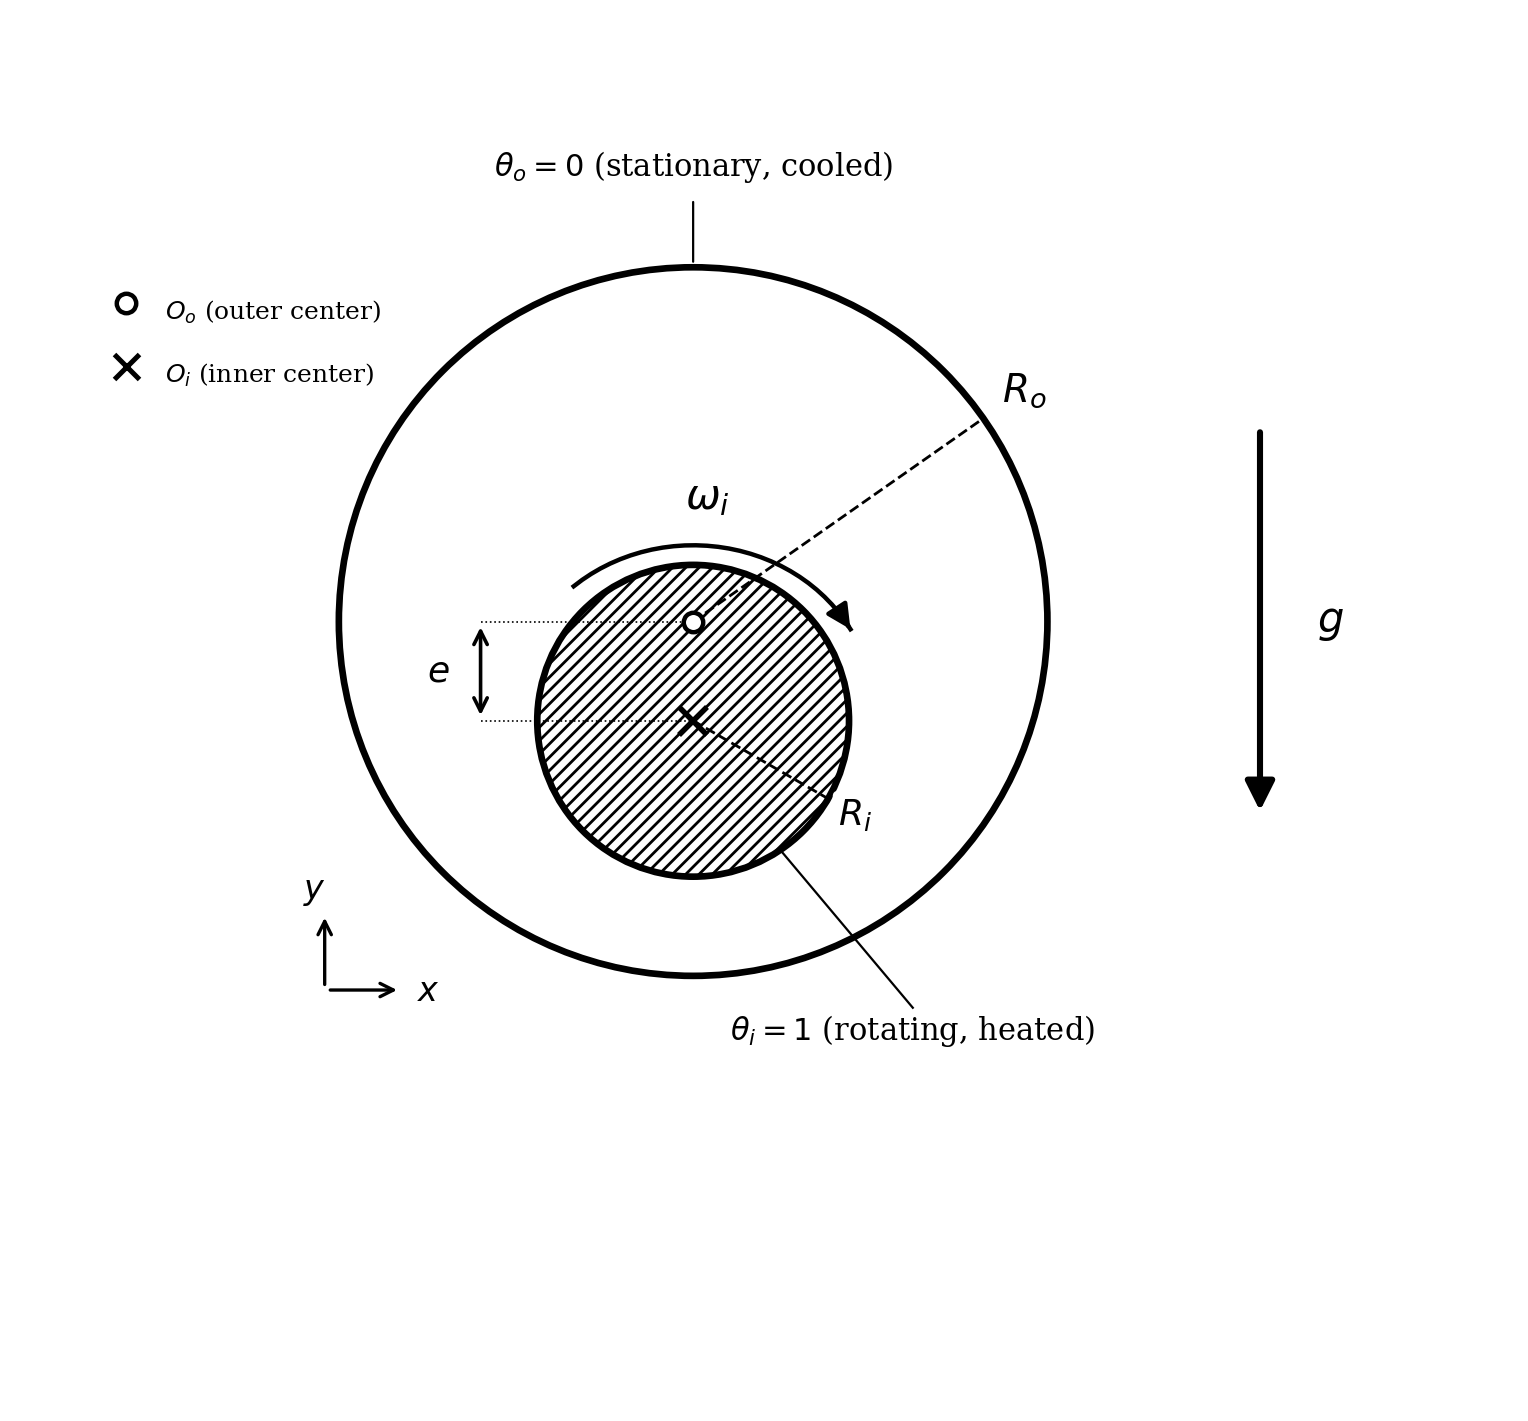
\includegraphics[width=0.90\textwidth]{figures/fig_schematic}
\caption{Schematic of the physical configuration: an eccentric horizontal annulus with a stationary, cooled outer cylinder ($\theta_o = 0$, radius $R_o$) and a rotating, heated inner cylinder ($\theta_i = 1$, radius $R_i$, angular speed $\omega_i$), offset from the outer cylinder's center by eccentricity $e$.}
\label{fig:schematic}
\end{figure}

\subsection{Governing Equations}
\label{subsec:governing}

Dimensional quantities are marked with a prime; the corresponding unprimed symbol is its non-dimensional counterpart. Position $\mathbf{x}'=(x',y')$, velocity $\mathbf{u}'=(u',v')$, time $t'$, pressure $p'$, temperature $T'$, and the inner wall's angular velocity $\omega'$ are non-dimensionalized using a reference length $L$ (the outer diameter), a reference velocity $U_{\text{ref}}=\omega_{\text{ref}}'L$ formed from a reference angular velocity $\omega_{\text{ref}}'$, and the imposed temperature difference $\Delta T' = T_i' - T_o'$:
\begin{equation}
  \mathbf{x} = \frac{\mathbf{x}'}{L}, \quad
  \mathbf{u} = \frac{\mathbf{u}'}{U_{\text{ref}}}, \quad
  t = \frac{t'U_{\text{ref}}}{L}, \quad
  p = \frac{p'}{\rho' U_{\text{ref}}^2}, \quad
  \theta = \frac{T' - T_o'}{\Delta T'}, \quad
  \omega = \frac{\omega'}{\omega_{\text{ref}}'},
  \label{eq:nondim_vars}
\end{equation}
with reference density $\rho'$, specific heat $c_p'$, gravitational magnitude $g'$, reference length $L$, and $\Delta T'$ all set to unity in the units used to solve the problem, so that $U_{\text{ref}}$ carries the correct dimension of velocity, $[\text{length}][\text{time}]^{-1}$, given that $\omega_{\text{ref}}'$ has dimension $[\text{time}]^{-1}$ (the radian itself is dimensionless). Under these definitions, the non-dimensional governing equations under the Boussinesq approximation are

\begin{equation}
  \nabla \cdot \mathbf{u} = 0,
  \label{eq:continuity}
\end{equation}
\begin{equation}
  \frac{\partial \mathbf{u}}{\partial t} + (\mathbf{u}\cdot\nabla)\mathbf{u} = -\nabla p + \frac{1}{Re} \nabla^2 \mathbf{u} + Ri\,\theta\,\hat{\mathbf{g}},
  \label{eq:momentum}
\end{equation}
\begin{equation}
  \frac{\partial \theta}{\partial t} + (\mathbf{u}\cdot\nabla)\theta = \frac{1}{Re\,Pr} \nabla^2 \theta,
  \label{eq:energy}
\end{equation}

where $\mathbf{u}=(u,v)$ is the non-dimensional velocity, $\theta$ the non-dimensional temperature, and $\hat{\mathbf{g}}=(0,-1)$ the unit vector in the direction of gravity (unrelated to the prime/unprimed dimensional notation above). $Re = U_{\text{ref}}L/\nu'$ is the Reynolds number and $Ri = Gr/Re^2$ the Richardson number, with $Gr = g'\beta'\Delta T' L^3/\nu'^2$ the Grashof number and $\nu'$, $\beta'$ the dimensional kinematic viscosity and thermal expansion coefficient; $Ra = Gr\,Pr$ recovers the Rayleigh number used in the classical annulus-convection literature and is reported throughout as a derived quantity for that purpose.

The reference length is fixed at $L=1$, common to all 35 geometries, rather than the physical gap width, which varies from case to case; this keeps the parameter sweep internally self-consistent but differs from the classical convention, which non-dimensionalizes using the gap width $L = R_o - R_i$~\cite{KuehnGoldstein1978,Lee1992a,Lee1992b,Yoo1998}. The conversion applied whenever a direct numerical comparison against that literature is made is given below.

The inner wall's rotation rate is fixed at a single non-dimensional value, $\omega_i=1$ (that is, $\omega_{\text{ref}}'$ is chosen equal to the inner wall's own dimensional rotation rate $\omega_i'$ for every case), rather than swept as an independent parameter, a choice that follows directly from the physics of a single rotating cylinder rather than being an arbitrary simplification. For one rotating boundary (as opposed to two independently-rotating cylinders, where the ratio between their rates is itself a physically meaningful, independent parameter), the rotational contribution to the flow is fully captured by $Re$; sweeping $\omega_i$ and viscosity independently would be redundant, since many dimensional $(\omega_i',\nu')$ pairs collapse onto the same $Re$. With $U_{\text{ref}}=\omega_i'L$, $Re$ reduces to $Re=1/\nu$ (the non-dimensional viscosity $\nu=\nu'/(U_{\text{ref}}L)$), so $Re$ is controlled directly and solely through viscosity, at fixed $Pr=0.71$ throughout (the corresponding solver implementation is described in the CFD methodology below). $Gr$, and therefore $Ri$, is controlled through the thermal expansion coefficient; with $L=1$ and $\omega_i=1$ as above, $Ri$ reduces to $Ri=\beta$ (the non-dimensional thermal expansion coefficient) exactly, independent of geometry, viscosity, or $Re$ (the derivation is straightforward substitution into the definitions above and was additionally confirmed numerically before use).

The four inputs used throughout this study, including as the machine learning surrogate's input feature set, are therefore the radius ratio $R^\ast = R_i/R_o$ (swept from 0.1 to 0.6 across 35 geometries), the eccentricity $\varepsilon$ (swept from 0 to a geometry-dependent maximum), the Reynolds number $Re$ (swept from 10 to 1000 across 12 log-spaced levels), and the Richardson number $Ri$ (swept from 0.01 to 10 across 13 levels, deliberately densified near $Ri\sim1$, the mixed-convection transition where buoyancy and rotation are comparably important). They are independent by construction: geometry is set through the mesh, $Re$ through viscosity, and $Ri$ through the thermal expansion coefficient, with the inner wall's rotation rate itself held fixed as derived above.

\subsection{Boundary Conditions}
\label{subsec:bc}

\begin{equation}
\begin{array}{lll}
  \theta = 0,\; u=v=0 & r = R_o & \text{(outer wall, stationary)} \\[4pt]
  \theta = 1,\; \mathbf{u} = \omega_i\,\hat{\mathbf{z}}\times(\mathbf{r}-\mathbf{r}_c) & r = R_i,\ \mathbf{r}_c=(0,-e) & \text{(inner wall, rotating)}
\end{array}
\label{eq:bc}
\end{equation}

The outer wall is a stationary no-slip boundary, $u=v=0$ in the lab-fixed frame. The inner wall is a rigidly rotating no-slip boundary: no-slip there means the fluid velocity matches the wall's own local velocity, $\omega_i\,\hat{\mathbf{z}}\times(\mathbf{r}-\mathbf{r}_c)$, the non-dimensional tangential velocity field of a rigid body rotating at rate $\omega_i$ about its center $\mathbf{r}_c=(0,-e)$, not zero. Because $\omega_i=1$ identically for every case in this study, as derived above, $\omega_i$ never appears as a free parameter in Equation~\eqref{eq:bc}; it is retained symbolically here only to keep the boundary condition dimensionally general.

\subsection{Nusselt Number Definition and Classical-Convention Conversion}
\label{subsec:nu_convention}

The Nusselt number reported throughout the dataset generation is $Nu = q''/k$, the area-weighted average heat flux on the inner wall divided by the thermal conductivity. This convention is internally consistent across the 35-geometry sweep, but, unlike the classical literature convention, it is not normalized to the pure-conduction limit and does not approach unity as $Ra \to 0$.

The classical convention~\cite{KuehnGoldstein1978,Lee1992a,Lee1992b,Yoo1998,Pranowo2024} instead defines $Nu_{\text{classical}}$ as the ratio of the actual to the pure-conduction heat transfer, so that $Nu_{\text{classical}} \to 1$ as $Ra \to 0$. Converting between the two conventions requires

\begin{equation}
  Ra_{\text{classical}} = Ra \times (R_o - R_i)^3, \qquad
  Nu_{\text{classical}} = Nu \times \frac{2\pi R_i}{S},
  \label{eq:conversion}
\end{equation}

where $S$ is the pure-conduction shape factor. For the concentric case, $S = 2\pi/\ln(R_o/R_i)$, the standard result. For the eccentric case,

\begin{equation}
  S = \frac{2\pi}{\operatorname{arccosh}\!\left(\dfrac{R_i^2+R_o^2-e^2}{2 R_i R_o}\right)},
  \label{eq:shape-factor}
\end{equation}

the bipolar-coordinate solution to Laplace's equation for two non-concentric isothermal circular boundaries, which reduces to the concentric formula as $e\to0$. Equation~\eqref{eq:shape-factor} was derived independently in this work and confirmed by a direct (non-iterative) sparse-matrix solution of Laplace's equation on the immersed-boundary annular domain, at four eccentric test geometries and five successively refined grids ($151^2$ to $1{,}201^2$); the numerical result converges monotonically toward the closed form at every geometry as resolution increases (from $1.5$--$3.4\%$ at the coarsest grid to $0.24$--$0.44\%$ at the finest), the signature of genuine grid convergence toward the analytical answer rather than a coincidental match. It was further shown to be algebraically identical to the closed-form result obtained by Prusa and Yao~\cite{PrusaYao1983} via conformal transformation, an independent derivation route. This three-way agreement, first-principles derivation, grid-converged numerical solution, and an independently published closed-form result obtained by a different method, is the strongest single methodological confirmation in the validation effort reported below.

\section{Computational Fluid Dynamics Methodology}
\label{sec:cfd}

\subsection{Solver and Discretization}
\label{subsec:solver}

The governing equations~\eqref{eq:continuity}--\eqref{eq:energy} subject to boundary conditions~\eqref{eq:bc} were solved using the commercial finite-volume solver ANSYS Fluent 2026 R1, driven programmatically through the PyFluent Python interface. The SIMPLE algorithm was employed for pressure-velocity coupling, with PRESTO! pressure discretization and Fluent's default second-order-upwind discretization for the momentum and energy equations. The Boussinesq density model was activated to account for buoyancy-driven flow, with air ($Pr=0.71$) as the working fluid. $Pr$ was held fixed at $0.71$ for every run, independent of the viscosity value used to set $Re$, by setting the thermal conductivity input as $k=\nu/Pr$ per run rather than fixing it at a single value; without this, holding conductivity fixed while varying viscosity alone would let $Pr$ float with $Re$ and never reach air's physical value.

\subsection{Computational Domain and Mesh}
\label{subsec:mesh}

Each of the 35 geometries was meshed independently, with 1,700 to 7,300 cells depending on geometry, using inflation layers at both the inner and outer walls to resolve the near-wall thermal and momentum boundary layers. Figure~\ref{fig:mesh} shows the production mesh for a representative geometry ($R^\ast=0.3$, $\varepsilon=0$, case 16, the geometry used for the mesh-independence study below): (a) the full domain and (b) a detailed view spanning from the inner wall's inflation layers to the outer boundary. Each raw mesh file additionally contains an unintended, fully enclosed disk of cells filling the inner cylinder itself, a legacy artifact of the sketch-based geometry construction (confirmed via Fluent's own mesh-check utility: total cell area exceeds the true annulus area, $\pi(R_o^2-R_i^2)$, by an amount matching a full disk of radius $R_i$ to within $1\%$). This disk is walled off from the annulus by a genuine wall/shadow face pair and is decoupled from it by the explicit one-sided \texttt{Temperature} thermal condition set on the inner wall, described above, which is the primary basis for treating it as harmless: the solver never couples across a Dirichlet boundary condition regardless of what lies on its far side. This is corroborated, though not independently proven, by the reasonable quantitative agreement with the Kuehn and Goldstein experimental data reported below; a mesh artifact leaking heat into the domain would be expected to bias that comparison in a specific, systematic direction, which is not observed. The disk is excluded from Figure~\ref{fig:mesh} as not part of the physical fluid domain.

\begin{figure}[h]
\centering
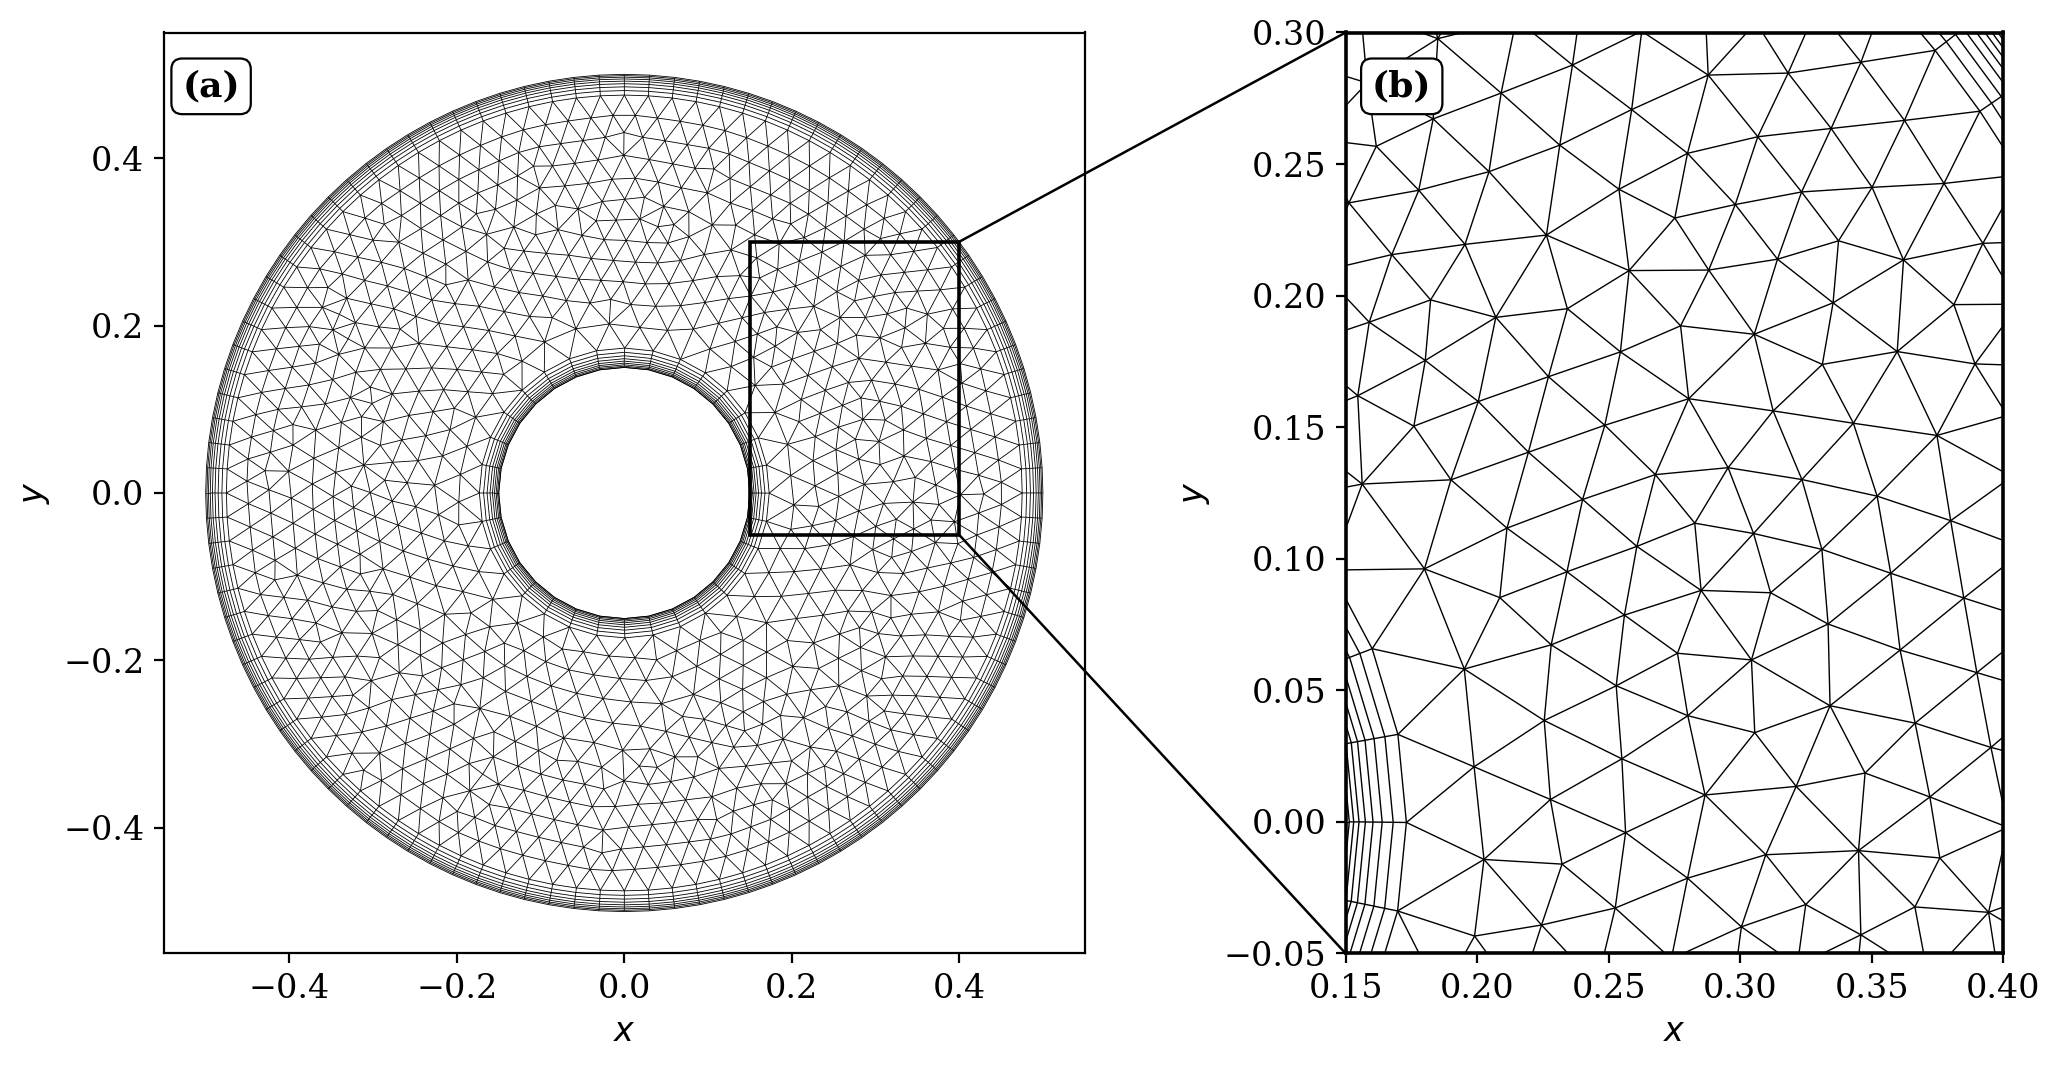
\includegraphics[width=\textwidth]{figures/fig_mesh}
\caption{Computational mesh for a representative geometry ($R^\ast=0.3$, $\varepsilon=0$); the unintended interior disk described in the text is excluded. (a) Full domain, 2,351 nodes, 5,538 faces. (b) Detail spanning the inner wall's 8-layer inflation stack, its transition into the bulk triangulation, and the outer boundary.}
\label{fig:mesh}
\end{figure}

Grid independence was reassessed for the present Re/Ri parameterization at this same geometry, using the same three systematically refined meshes as the initial study (coarse/medium/fine, unchanged, since the meshes themselves depend only on geometry, not on how the physics is parameterized), at a moderate mixed-convection operating point, $Re=100$, $Ri=1$ ($Ra\approx7{,}100$), via the Grid Convergence Index (GCI) procedure of Celik et al.~\cite{Celik2008} (Table~\ref{tab:gci}). The apparent order of convergence is $p=1.83$, the fine-grid GCI is $0.18\%$, and the asymptotic-range indicator evaluates to $1.001$, confirming the production mesh lies within the asymptotic grid-convergence regime at this representative point. A moderate operating point was chosen deliberately over the sweep's most extreme corner ($Re=1000$, $Ri=10$, $Ra\approx7.1\times10^6$): an initial attempt at that corner gave a non-monotonic mesh dependence ($Nu=$ 23.87, 23.71, 24.13 for coarse/medium/fine), which violates the GCI procedure's assumption of monotone convergence and most likely reflects genuine physical unsteadiness onsetting near the top of the simulated $Ra$ range (independent evidence noted above indicates that $Ra\sim10^6$ sits near the edge of steady-laminar validity for this problem class) rather than a discretization-error signal a steady-state GCI analysis can meaningfully quantify. A separate, simpler adequacy check was instead performed at that extreme corner directly: comparing the production mesh against a substantially refined mesh (15 boundary layers at a $0.0004$ first-layer height vs.\ the production mesh's 8 layers at $0.0015$, at $R^\ast=0.1$) gave a $Nu$ difference of $0.24\%$, supporting adequacy at the extreme corner without relying on the (here inapplicable) formal asymptotic-order machinery.

\begin{table}[h]
\centering
\caption{Grid Convergence Index (GCI) analysis following Celik et al.~\cite{Celik2008}, at $R^\ast=0.3$, $\varepsilon=0$, $Re=100$, $Ri=1$ ($Ra\approx7{,}100$).}
\label{tab:gci}
\begin{tabular}{lc}
\toprule
Quantity & Value \\
\midrule
Coarse mesh & 1{,}758 cells, $Nu_3 = 5.57566$ \\
Medium (production) mesh & 3{,}188 cells, $Nu_2 = 5.58640$ \\
Fine mesh & 6{,}300 cells, $Nu_1 = 5.59327$ \\
Refinement ratio $r_{21}$ & 1.406 \\
Refinement ratio $r_{32}$ & 1.347 \\
Apparent order of convergence, $p$ & 1.833 \\
Richardson-extrapolated value, $Nu_\text{ext}$ & 5.60119 \\
Approximate relative error, $e_{21}$ & 0.123\% \\
Extrapolated relative error, $e_\text{ext}$ & 0.142\% \\
Fine-grid GCI, $\text{GCI}_\text{fine}^{21}$ & \textbf{0.177\%} \\
Medium-grid GCI, $\text{GCI}_\text{medium}^{32}$ & 0.331\% \\
Asymptotic-range indicator & 1.001 \\
\bottomrule
\end{tabular}
\end{table}

\subsection{Convergence Criteria}
\label{subsec:convergence}

Rather than iterating every case to a single fixed iteration count and residual target, each case was run for a base 1,000 iterations and then advanced in further blocks of 500, re-evaluating the area-averaged Nusselt number after each block; a case was accepted once two successive block-end $Nu$ values agreed to within $0.3\%$, and abandoned as non-converged if this stability criterion was not met within a ceiling of 6,000 iterations. This adaptive scheme was adopted specifically because the achieved Rayleigh number now varies by more than four orders of magnitude across the sweep; a single iteration budget tuned for the low end of that range cannot be assumed adequate at the high end without checking, and checking per case, rather than assuming, was judged the more defensible approach. Both the convergence flag and the total iteration count are recorded per case in the released dataset. Of the 5,460 production simulations, all 5,460 (100\%) reached this criterion within the allotted budget; none were dropped from the machine learning dataset.

\subsection{Code Validation}
\label{subsec:cfd_val}

Because no single published source reports Nusselt number as a function of the full joint $(R^\ast, \varepsilon, Re, Ri)$ parameter space studied here, validation was assembled from four independent, complementary lines of evidence.

Kuehn and Goldstein~\cite{KuehnGoldstein1978} report 39 experimentally measured heat-transfer points for a concentric, stationary annulus with a fixed diameter ratio of 2.6, spanning $Ra_L = 2.2\times10^2$ to $7.7\times10^7$. Their reported quantity, $\bar k_{eq} = Nu/Nu_{\text{cond}}$, is identical in definition to the classical-convention Nusselt number defined above. Sixteen of their tabulated $Ra_L$ values fall within the range reachable at the present nearest-matching geometry ($R^\ast=0.4$, diameter ratio 2.5 vs.\ their 2.6) and weakest available rotation ($Re=10$); rather than interpolate the present results onto their grid, the thermal expansion coefficient was chosen for sixteen dedicated runs so that the present $Ra_L$ (gap-width convention, Equation~\eqref{eq:conversion}) lands exactly on each of their sixteen values, giving a direct point-for-point comparison with no interpolation on either side. Across these sixteen points the mean absolute difference is $5.3\%$ and the maximum is $9.8\%$ (Table~\ref{tab:validation}, Figure~\ref{fig:kg-comparison}), within the $1.6$--$8.3\%$ spread reported between independent numerical and experimental studies of this same benchmark case~\cite{Pranowo2024}. The difference is small and smoothly varying with $Ra_L$ rather than randomly scattered (near-zero below $Ra_L\approx10^3$, drifting to approximately $-9\%$ above $Ra_L\approx3\times10^4$), consistent with the two known, physically legitimate sources of residual disagreement: the $4\%$ geometry mismatch, and the present comparison's non-zero rotation ($Re=10$) against Kuehn and Goldstein's purely stationary experiment, which Lee~\cite{Lee1992a,Lee1992b} (discussed next) establishes should suppress $Nu$ somewhat relative to the stationary case.

\begin{table}[h]
\centering
\small
\caption{Validation against the experimental data of Kuehn and Goldstein~\cite{KuehnGoldstein1978}, nearest matching geometry $R^\ast=0.4$ (diameter ratio 2.5 vs.\ their 2.6), $Re=10$. The present $Ra_L$ was chosen (via the thermal expansion coefficient) to match each experimental value exactly; both columns report the same dimensionless quantity, the ratio of actual to pure-conduction heat transfer ($Nu_{\text{classical}} = \bar k_{eq}$ by definition).}
\label{tab:validation}
\begin{tabular}{cccc}
\toprule
$Ra_L$ & Experiment~\cite{KuehnGoldstein1978} & Present (CFD) & Relative error \\
\midrule
$221$ & 5.293 & 5.469 & $+3.3\%$ \\
$496$ & 5.457 & 5.560 & $+1.9\%$ \\
$544$ & 5.566 & 5.583 & $+0.3\%$ \\
$826$ & 5.784 & 5.750 & $-0.6\%$ \\
$1{,}310$ & 6.221 & 6.131 & $-1.4\%$ \\
$2{,}380$ & 7.530 & 7.083 & $-5.9\%$ \\
$3{,}660$ & 8.349 & 8.047 & $-3.6\%$ \\
$5{,}910$ & 9.931 & 9.269 & $-6.7\%$ \\
$9{,}500$ & 10.968 & 10.569 & $-3.6\%$ \\
$12{,}900$ & 12.278 & 11.447 & $-6.8\%$ \\
$20{,}800$ & 13.478 & 12.875 & $-4.5\%$ \\
$32{,}000$ & 15.770 & 14.232 & $-9.8\%$ \\
$61{,}900$ & 18.117 & 16.442 & $-9.2\%$ \\
$102{,}000$ & 19.972 & 18.296 & $-8.4\%$ \\
$144{,}000$ & 21.663 & 19.719 & $-9.0\%$ \\
$225{,}000$ & 23.955 & 21.742 & $-9.2\%$ \\
\midrule
\multicolumn{3}{l}{Mean absolute relative error} & \textbf{5.3\%} \\
\multicolumn{3}{l}{Maximum absolute relative error} & \textbf{9.8\%} \\
\bottomrule
\end{tabular}
\end{table}

\begin{figure}[h]
\centering
\includegraphics[width=\textwidth]{../03-computation/validation/re_ri_dataset/validation_vs_kuehngoldstein_final.png}
\caption{Nusselt number, converted to the classical convention, compared against sixteen exactly-matched-$Ra_L$ experimental points of Kuehn and Goldstein~\cite{KuehnGoldstein1978} (left: overlaid curves; right: relative difference vs.\ $Ra_L$, shaded band $\pm10\%$). Mean absolute difference $5.3\%$, maximum $9.8\%$.}
\label{fig:kg-comparison}
\end{figure}

Lee~\cite{Lee1992a,Lee1992b} report, in text, that the mean Nusselt number decreases monotonically with rotational Reynolds number at fixed $Ra$, at a rate that depends on eccentricity. This was checked directly against the present dataset by searching for pairs of simulations with exactly-matching $Ra$ (to within $0.1\%$) achieved via different $(Re,Ri)$ combinations. At low $Ra$ ($<3{,}000$, conduction-dominated), all such pairs agreed to within $0.01\%$, inside the dataset's own $0.3\%$ convergence tolerance and therefore inconclusive by construction, as expected since there is little real convection at those conditions for rotation to suppress. At $Ra=7{,}100$, within the convective regime, $Nu$ decreased by a clean $0.6\%$ as $Re$ increased from 50 to 1000 at fixed $Ra$, well above the noise floor and in the direction Lee's finding predicts.

A further independent numerical study of the same concentric benchmark geometry, Fusegi et al.~\cite{Fusegi1986}, corroborates the Kuehn and Goldstein dataset visually and additionally reports mixed convection with a heated rotating inner cylinder using the same rotational parameter, $Gr/Re^2$, adopted here as $Ri$, though its results are reported only graphically and were not re-digitized for a numeric comparison.

The three checks above all involve buoyancy; a fourth, independent check isolates the rotational momentum boundary condition alone. With buoyancy switched off entirely (gravity disabled, decoupling momentum from temperature) and the inner wall rotating at a non-dimensional rate $\Omega=10$, deliberately distinct from the main study's fixed $\omega_i=1$ and chosen only for this standalone check, about a concentric ($e=0$) geometry, the resulting flow is pure circular Couette flow, with an exact closed-form solution, $v_\theta(r) = Ar+B/r$, $A=\Omega R_i^2/(R_i^2-R_o^2)$, $B=-AR_o^2$, obtainable directly from the momentum equation with no free parameters to fit. Comparing this solution against the CFD result at every interior mesh node (excluding both the walled-off inner-disk artifact and the wall boundary nodes themselves, whose exported velocity is reported relative to the moving wall and is therefore trivially zero by no-slip, not a discrepancy) gives a root-mean-square difference of $0.55\%$ and a maximum difference of $1.16\%$ of the wall speed, confirming that the rotating-wall boundary condition and momentum solver reproduce the exact rotational solution independent of, and prior to, any buoyancy coupling, following the same isothermal-limit validation logic used by Yoo~\cite{Yoo1998} for the reversed (rotating-outer) configuration.

\section{Dataset Generation and Surrogate Model Inputs}
\label{sec:dataset}

\subsection{Parametric Study Design}
\label{subsec:params}

Thirty-five geometries were generated, spanning six radius-ratio groups ($R^\ast = 0.1,\allowbreak\ 0.2,\ 0.3,\ 0.4,\ 0.5,\ 0.6$), each swept over a group-dependent range of eccentricities from zero to a maximum set by physical clearance; these 35 geometries are unchanged from the initial study design. Each geometry was solved across twelve Reynolds numbers ($Re = 10$ to $1000$, log-spaced) and thirteen Richardson numbers ($Ri = 0.01$ to $10$, densified near $Ri\sim1$), giving $35 \times 12 \times 13 = 5{,}460$ total simulations (Table~\ref{tab:params}). All 5,460 satisfied the adaptive convergence criterion described above; none were dropped, so all 5,460 cases were used for surrogate model training.

\begin{table}[h]
\centering
\caption{Governing parameters, ranges, and design levels for the CFD dataset.}
\label{tab:params}
\begin{tabular}{lccc}
\toprule
Parameter & Symbol & Range & Levels \\
\midrule
Radius ratio      & $R^\ast$   & $[0.1,\ 0.6]$   & 6 groups (35 geometries total) \\
Eccentricity      & $\varepsilon$ & $[0,\ \varepsilon_{\max}(R^\ast)]$ & 5--8 per group \\
Reynolds number   & $Re$       & $[10,\ 1000]$   & 12 \\
Richardson number & $Ri$       & $[0.01,\ 10]$   & 13 \\
\bottomrule
\end{tabular}
\end{table}

\subsection{Output Variables}
\label{subsec:output}

Two outputs were recorded per simulation: the scalar area-averaged Nusselt number on the inner wall, used to train the scalar surrogate, and, separately, the full spatial field of temperature and velocity at every mesh node, used to train the spatial field surrogate.
